\documentclass[journal]{IEEEtran}
\usepackage[T1]{fontenc}
\usepackage[utf8]{inputenc}
\usepackage{amsmath,amssymb}
\usepackage{xcolor}
\usepackage{graphicx}
\usepackage{cite}
\usepackage{booktabs}
\usepackage{threeparttable}
\usepackage{tikz}
\usetikzlibrary{arrows.meta,positioning,calc,fit,backgrounds}
\usepackage[hidelinks]{hyperref}

\newtheorem{proposition}{Proposition}
\newtheorem{corollary}{Corollary}

% Red marks text that waits on runs still in progress (ASGNet) or on a decision.
% Remove the colour before submission.
\newcommand{\pend}[1]{\textcolor{red}{#1}}

\begin{document}

\title{Which View Should Teach? Label-Aware Flip Consistency for Generalizable Polyp Segmentation}
\author{\pend{Authors}}
\maketitle

\begin{abstract}
Polyp segmentation networks lose accuracy on centres unseen in training. A mirrored
polyp is still a polyp, so a reliable model should predict the mirrored mask for a
mirrored image; we observe that trained models do not, and are least flip-consistent on
the hardest test sets. Flip consistency regularization is a natural remedy, but it comes
from semi-supervised learning, where no label says which view is correct. We show that,
in binary segmentation with labels available, a cross-entropy consistency pull toward a
teacher view is a reweighted supervised pull: it moves the student view toward the label
only where the teacher is closer to it. Building on this identity, we propose label-aware
flip-consistency training (FCT), in which each view is pulled at full strength only
toward a more accurate view, and never toward a misclassification it has avoided. The
rule's one constant is set by the decision threshold rather than tuned, and FCT leaves
the network and its inference unchanged. Experiments on five public benchmarks, each repeated over six random seeds, show that
FCT improves the five-set mean Dice of Polyp-PVT and PraNet-V2 on every seed
\pend{[ASGNet: pending]} and markedly reduces flip inconsistency. Notably, on the unseen ETIS dataset, FCT improves PraNet-V2 by 3.6 Dice
points. \pend{Code is available at [URL].}
\end{abstract}

\begin{IEEEkeywords}
Polyp segmentation, domain generalization, consistency regularization, flip equivariance,
self-distillation.
\end{IEEEkeywords}

\section{Introduction}
\label{sec:intro}

Polyp segmentation networks that are accurate on their training data lose much of that accuracy
at new centres, whose images differ in endoscopes, illumination and
patients~\cite{ali2023polypgen,ali2024endocv}. This gap limits their clinical value: colorectal
cancer is among the leading causes of cancer death~\cite{siegel2024cancer}, and automatic
segmentation aims to help endoscopists, who miss about one in five
polyps~\cite{vanrijn2006miss}. Recent networks reach high Dice on test images from their
training datasets~\cite{fan2020pranet,wei2021sanet,dong2023polyppvt,hu2026pranetv2,sun2026asgnet},
but much lower Dice elsewhere. In our experiments, for example, Polyp-PVT~\cite{dong2023polyppvt}
reaches 93.2\% mean Dice on \mbox{CVC-ClinicDB} but only 78.6\% on ETIS, a dataset from another
hospital. For clinical use, closing this gap matters more than further gains on the training
distribution.

Polyp segmentation also has a symmetry that standard training does not enforce. A mirrored
polyp is still a polyp, so the correct mask of a mirrored image is the mirrored mask. We measure
departures from this flip equivariance with the flip gap: one minus the Dice overlap between the
binary masks predicted for an image and for its flipped copy, once flipped back, averaged over
horizontal and vertical flips. As Fig.~\ref{fig:teaser} shows, the flip gap of trained models
is far from zero, and it is largest on the two hardest test sets, \mbox{CVC-ColonDB} and ETIS.
We hypothesize that a model whose answer changes with a mirror image relies partly on cues that
do not belong to the polyp, and that such cues are unlikely to transfer to new centres.

\begin{figure*}[t]
\centering
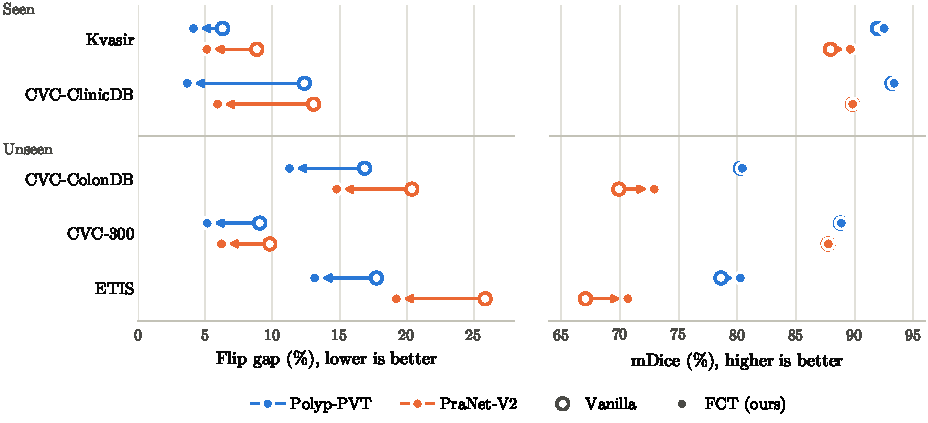
\includegraphics[width=\textwidth]{figures/fig1_flipgap.pdf}
\caption{Flip gap (left; one minus the Dice overlap between the binary masks predicted for an
image and for its flipped copy, once flipped back, averaged over horizontal and vertical flips)
and mDice (right) on five test sets, without (hollow) and with (filled) FCT. Both networks are
least flip-consistent on \mbox{CVC-ColonDB} and ETIS, the two sets where they are least
accurate. FCT lowers the flip gap on every set, and its largest mDice gain, for both networks,
is on ETIS. Means over six seeds.}
\label{fig:teaser}
\end{figure*}

Two remedies are common, and both act on the training loss. Flip augmentation trains on mirrored
copies with mirrored labels, but each copy is constrained only by its own label, never by the
prediction on its mirror. Consistency regularization adds that constraint with a loss term that
penalizes disagreement between the predictions on the views. It comes from semi-supervised
learning, where agreement between views is the only signal that unlabeled images
provide~\cite{laine2017temporal,tarvainen2017mean,sohn2020fixmatch}, and medical variants enforce it
under spatial transformations~\cite{bortsova2019consistency,li2021tcsm}. Since no label says which
view is right, the views are treated as equally reliable or weighed by the model's own confidence.
Supervised uses of consistency, such as AugMix~\cite{hendrycks2020augmix} and
R-Drop~\cite{liang2021rdrop}, keep this symmetry even though the label is known, so a correct view
can be drawn toward a wrong one.

We show that, under full supervision, a consistency term is a reweighted supervised loss. For binary
segmentation, the gradient of a cross-entropy consistency term that draws one view toward the detached
prediction of another equals the supervised gradient, scaled by one minus the ratio of the two views'
errors. Similar decompositions of the distillation gradient are known for
classification~\cite{furlanello2018born,tang2020understanding}; here we apply the identity pixel by
pixel, across views of one image. A consistency term is therefore an adaptive pixel weight on the
supervised loss: positive where a view is farther from the label than its target, and negative where
it is closer. Unweighted consistency mixes both kinds of pixels in every image, and only the label
can tell them apart.

Building on this identity, we propose flip-consistent training (FCT), a plug-in training loss for
polyp segmentation. FCT supervises each image in three orientation views, upright, flipped
horizontally and flipped vertically, and adds a consistency term that draws the predictions of the
views together: each flipped view toward the upright view, and the upright view toward the flipped view
closest to the label. Label-aware weights complete the loss. A flipped view moves toward the upright
view at full strength where it is farther from the label; where it is closer, it moves only if the
upright view is correct, in proportion to how far the upright prediction lies on the correct side of
the 0.5 threshold. This weak term keeps the views consistent without moving either across the
threshold, much as label smoothing tempers overconfident targets~\cite{yuan2020revisiting}, and its
single constant is set by the decision threshold rather than tuned. FCT changes only the training
loss: it multiplies the training time by about 3.5 and adds nothing at inference. To the best of our
knowledge, FCT is the first consistency loss that uses the label to set, pixel by pixel, the
direction in which the views of an image are drawn together.

We add FCT, without retuning, to three segmentation networks of different design:
Polyp-PVT~\cite{dong2023polyppvt}, built on a pyramid vision transformer;
PraNet-V2~\cite{hu2026pranetv2}, a convolutional network with dual-supervised reverse attention;
and ASGNet~\cite{sun2026asgnet}, which guides its features with spectral cues and already trains
with random flips. Each network is trained with and without FCT under six paired random seeds and
tested on five public test sets, three of which are unseen in training. FCT improves ETIS for all
three networks, by +1.65, +3.61 and +1.69 points, and \mbox{CVC-ColonDB} for PraNet-V2, by +3.01
points, all with paired 95\% confidence intervals above zero. It raises the five-set mean Dice on
every seed for Polyp-PVT and PraNet-V2, and on five of six for ASGNet, whose gain is borderline. FCT
also lowers the five-set mean flip gap of Polyp-PVT and PraNet-V2 by 40\% and 34\%, respectively. On
six more centres from the PolypGen benchmark~\cite{ali2023polypgen}, a label-aware variant improves
the pooled Dice on every seed \pend{(FCT itself is pending)}. A study of the loss terms on Polyp-PVT
shows that the multi-view supervision accounts for most of the gain on ETIS, and that the consistency
term and its weights complete it: FCT is the only variant that improves all five test sets on
average \pend{(one row of the study is still running)}.

Our contributions are summarized as follows:
\begin{itemize}
\item We propose FCT, a plug-in training loss that supervises three orientation views of each image
and draws their predictions together with a label-weighted consistency term. It changes no
architecture and adds no cost at inference.
\item We show that, for binary labels, a consistency term between two views acts pixel by pixel as
the supervised loss with an adaptive weight, which is negative where a view is drawn toward a less
accurate one, and we derive label-aware weights whose single constant is set by the decision
threshold.
\item We evaluate FCT on three architectures, five test sets and six paired seeds with confidence
intervals, and dissect the loss into its terms. It improves ETIS for all three networks, raises the
five-set mean Dice on every seed for two of them, and makes the predictions of both markedly more
flip-consistent.
\end{itemize}

\section{Related Work}
\label{sec:related}

\subsection{Polyp Segmentation and Generalization}

Deep polyp segmentation has advanced mainly through network design.
PraNet~\cite{fan2020pranet} aggregates high-level features with a parallel partial decoder and
refines boundaries with reverse attention. SANet~\cite{wei2021sanet} adds shallow attention and
colour exchange, and UACANet~\cite{kim2021uacanet} attends to the uncertain region of each
prediction. Later networks adopt transformer encoders, as Polyp-PVT~\cite{dong2023polyppvt} and
ASGNet~\cite{sun2026asgnet} do, the latter guiding its features with spectral information, or
add supervision, as PraNet-V2~\cite{hu2026pranetv2} does with dual-supervised reverse attention.
Other recent designs add contrastive transformer modules~\cite{xiao2024ctnet}, boundary-sensitive
attention~\cite{shao2024polyper} or uncertainty modeling~\cite{du2025umnet}, or adapt the Segment
Anything Model with a convolutional branch~\cite{li2024asps}. Closest to our motivation,
VANet~\cite{cai2024vanet} observes that steering the colonoscope tip changes the viewpoint and the
appearance of polyps, and handles this with viewpoint-aware modules. These networks change the
architecture, whereas FCT changes only the training loss, so it complements rather than replaces
them.

Most of these models follow the protocol of~\cite{fan2020pranet}: they train on
Kvasir-SEG~\cite{jha2020kvasir} and CVC-ClinicDB~\cite{bernal2015clinicdb}, and they are tested
on these two datasets and on CVC-ColonDB~\cite{tajbakhsh2016colondb},
CVC-300~\cite{vazquez2017endoscene} and ETIS~\cite{silva2014etis}, which are unseen in training.
Accuracy on the unseen sets stays well below that on the seen ones, and multi-centre benchmarks
confirm the gap at scale~\cite{ali2023polypgen,ali2024endocv}. Domain generalization offers
training-side remedies~\cite{zhou2023dgsurvey}, such as shape-aware
meta-learning~\cite{liu2020saml} and frequency-space interpolation across
sites~\cite{liu2021feddg}. For polyps, randomized global illumination
augmentation~\cite{zhang2024illumination} and colour transfer~\cite{du2025umnet} target nuisance
factors that vary across centres, and domain adaptation learns from unlabeled images of the target
domain~\cite{lu2025dclps}. These methods diversify the training data, learn from differences
between domains or need target images, whereas FCT adds a constraint between views of each training
image and needs no target data, so the approaches are complementary.

\subsection{Consistency Regularization and Equivariance}

Consistency regularization asks a network to agree with itself across perturbed views of an
input. It was developed for semi-supervised learning, where unlabeled images provide only this
signal: the $\Pi$-model and temporal ensembling~\cite{laine2017temporal}, mean
teachers~\cite{tarvainen2017mean}, unsupervised data augmentation~\cite{xie2020uda} and
FixMatch~\cite{sohn2020fixmatch}. FixMatch keeps only pseudo-labels whose confidence exceeds a
threshold, a proxy for correctness when the true label is unknown. Semi-supervised segmentation
methods perturb inputs, features or networks~\cite{ouali2020cct,chen2021cps,yang2023unimatch}.
In medical imaging, consistency under spatial transformations exploits the equivariance of
segmentation on unlabeled scans~\cite{bortsova2019consistency,li2021tcsm}, or its invariance to
the surrounding context~\cite{liu2025tracoco}. Mean teachers restrict consistency to reliable
regions~\cite{yu2019uamt} or to ambiguous ones~\cite{xu2023acmt}, bidirectional patch displacement
builds new samples for consistency learning guided by prediction confidence~\cite{chi2024abd}, and
semi-supervised polyp segmentation aligns the affinity maps of a student and a
teacher~\cite{wu2023aclnet}.

With labels available, consistency also serves as a regularizer: AugMix~\cite{hendrycks2020augmix}
matches predictions across augmentation chains, and R-Drop~\cite{liang2021rdrop} across dropout
masks. A sample-efficiency analysis shows that, with label-invariant augmentations, consistency
regularization learns from fewer samples than training on the augmented copies with their
labels~\cite{yang2023dac}. Flip and rotation augmentation, by contrast, supervises each transformed copy with its own
transformed label and does not relate the predictions on different copies. Equivariance can also
be built into the architecture~\cite{cohen2016gcnn,veeling2018rotation}, enforced on class
activation maps in weakly supervised segmentation~\cite{wang2020seam}, or approximated at test
time by averaging predictions over transformed inputs~\cite{wang2019tta}, at the price of a
constrained architecture or a multiplied inference cost. All these methods treat the views as
equally reliable or weigh them by the model's own confidence, since none uses the label to
compare views; under full supervision, FCT does exactly that.

\subsection{Self-Distillation and Label-Aware Weighting}

Knowledge distillation trains a student to match the soft predictions of a
teacher~\cite{hinton2015distilling}. In self-distillation, the teacher is the model itself: an
earlier generation of the same architecture~\cite{furlanello2018born}, its own deeper
layers~\cite{zhang2019byot}, its predictions from the previous epoch~\cite{kim2021pskd} or
dropout-sampled versions of itself~\cite{lee2023sddropout}.
Closest to our setting, data-distortion guided self-distillation~\cite{xu2019ddgsd} makes a
network agree with itself on two distorted copies of an image under full supervision, treating
both copies alike. The consistency term of FCT is also self-distillation across views, but it
compares teacher and student against the label, pixel by pixel.

Several works relate distillation to the ground truth. Analyses of the distillation gradient
show that it rescales the supervised gradient according to the teacher's confidence in the true
class~\cite{furlanello2018born,tang2020understanding}, self-distillation over several rounds
averages the labels of instances with correlated features~\cite{jeong2025selfdistill}, and Yuan et
al.~\cite{yuan2020revisiting} relate distillation to label smoothing. Decoupled knowledge
distillation~\cite{zhao2022dkd} splits the loss exactly into target-class and non-target-class
terms, knowledge adjustment~\cite{wen2021preparing}, refined logits~\cite{sun2025rld} and label
revision~\cite{lan2025labelrevision} correct teacher predictions that contradict the label, and confidence-aware multi-teacher distillation~\cite{zhang2022camkd} weights each
teacher by how close its predictions are to the label. For segmentation, structured distillation
transfers pixel-wise and pairwise knowledge from a large network to a compact
one~\cite{liu2019skd}. Loss reweighting also changes how much
each example counts: focal loss~\cite{lin2017focal} and online hard example
mining~\cite{shrivastava2016ohem} emphasize examples with high loss, and the structure loss used
by PraNet-style networks emphasizes pixels near boundaries~\cite{wei2020f3net}. By our identity,
FCT belongs to this family: it reweights the supervised gradient of each pixel, but by how the
pixel's error compares with that of another view of the same pixel, within one network rather
than across separate teachers.

\section{Consistency as Reweighted Supervision}
\label{sec:analysis}

This section analyses the consistency term of a multi-view training loss. It shows that, when the
label is binary, a consistency term that draws one view toward the detached prediction of another
acts at every pixel as the supervised loss, rescaled by a factor that compares the errors of the
two views. The sign of this factor tells, pixel by pixel, whether the term helps or hurts, and
Section~\ref{sec:method} builds the weights of FCT on it.

\subsection{Notation}
\label{sec:notation}

Let $x\in\mathbb{R}^{H\times W\times 3}$ denote an image, $y\in\{0,1\}^{H\times W}$ its polyp mask,
and $f$ a segmentation network that maps $x$ to a logit map $z=f(x)\in\mathbb{R}^{H\times W}$; the
predicted probabilities are $p=\sigma(z)$, where $\sigma$ denotes the logistic function. Let $T_h$ and
$T_v$ denote the horizontal and vertical flips. Each flip is its own inverse, so the prediction for a
flipped view, brought back to the upright frame, is
\begin{equation}
z^{k}=T_k f(T_k x),\qquad k\in\{h,v\},
\label{eq:views}
\end{equation}
and the upright view gives $z^{o}=f(x)$. A flip-equivariant network satisfies $z^{h}=z^{v}=z^{o}$.
The flip gap of Section~\ref{sec:intro} measures departures from this equality on binary masks:
\begin{equation}
\Delta(x)=1-\frac{1}{2}\sum_{k\in\{h,v\}} D\big(\mathbf{1}[p^{o}>\tfrac12],\,\mathbf{1}[p^{k}>\tfrac12]\big),
\label{eq:flipgap}
\end{equation}
where $D$ denotes the Dice overlap of two masks and $\mathbf{1}[\cdot]$ the indicator function, applied
pixel by pixel.

At a pixel $i$, the error of a view is $e_i=|p_i-y_i|\in[0,1]$, and the view is correct at the
decision threshold of $\frac12$ if $e_i<\frac12$. We drop the index $i$ when a statement holds for
each pixel separately. A consistency term draws a view $s$ toward the prediction $p_t$ of a target
view $t$, which is detached, that is, treated as a constant. We write
\begin{equation}
\ell(z_s;q)=-q\log\sigma(z_s)-(1-q)\log\big(1-\sigma(z_s)\big)
\label{eq:bce}
\end{equation}
for the binary cross-entropy of the view's logit $z_s$ with a target $q\in[0,1]$. The consistency
term is $\ell(z_s;p_t)$ and the supervised loss is $\ell(z_s;y)$, and their gradients with respect to
the logit are
\begin{equation}
\frac{\partial\ell(z_s;p_t)}{\partial z_s}=p_s-p_t,\qquad
\frac{\partial\ell(z_s;y)}{\partial z_s}=p_s-y.
\label{eq:grads}
\end{equation}

\subsection{Consistency as an Adaptive Pixel Weight}
\label{sec:identity}

The two gradients in Eq.~\eqref{eq:grads} are parallel whenever the label is binary: the consistency
gradient is the supervised one, rescaled by how the errors of the two views compare.

\begin{proposition}
\label{prop:identity}
Let $y\in\{0,1\}$, $p_s,p_t\in[0,1]$ and $p_s\neq y$. Then
\begin{equation}
\frac{\partial\ell(z_s;p_t)}{\partial z_s}=\Big(1-\frac{e_t}{e_s}\Big)\frac{\partial\ell(z_s;y)}{\partial z_s},
\label{eq:identity}
\end{equation}
where $e_s=|p_s-y|$ and $e_t=|p_t-y|$ denote the errors of the view and of its target.
\end{proposition}

\begin{IEEEproof}
Because $y$ is $0$ or $1$, every $p\in[0,1]$ satisfies $p-y=(1-2y)|p-y|$: for $y=0$, $p-y=p$, and for
$y=1$, $p-y=-(1-p)$. Hence $p_s-p_t=(p_s-y)-(p_t-y)=(1-2y)(e_s-e_t)=(p_s-y)(1-e_t/e_s)$, where the last
step uses $(1-2y)e_s=p_s-y$ and $e_s>0$. Eq.~\eqref{eq:grads} completes the proof.
\end{IEEEproof}

The identity needs no assumption on the network or on the target's probability, only a binary
label, which places both errors on the same side of the target. It also holds for a squared-error
term on probabilities, whose gradient with respect to $p_s$ is again $p_s-p_t$. Summed over pixels
and differentiated with respect to the network parameters $\theta$, Eq.~\eqref{eq:identity} reads
\begin{equation}
\nabla_\theta\sum_i \ell(z_{s,i};p_{t,i})=\sum_i \omega_i\,\nabla_\theta\,\ell(z_{s,i};y_i),
\qquad \omega_i=1-\frac{e_{t,i}}{e_{s,i}},
\label{eq:weights}
\end{equation}
with the weights $\omega_i$ held constant. A consistency term is thus a supervised loss with
per-pixel weights, and some of these weights are negative.

When the view is also supervised, the two terms add. With a cross-entropy supervised term of weight
$\beta$ and a consistency term of weight $\gamma$, the gradient on the view's logit is
\begin{equation}
\big(\beta+\gamma\,\omega\big)\,(p_s-y),
\label{eq:combined}
\end{equation}
so the consistency term changes only how much each pixel's supervised gradient counts. Under full
supervision, it brings no information beyond the label: it acts as an adaptive pixel weight, as
focal loss~\cite{lin2017focal} and the structure loss~\cite{wei2020f3net} do, but set by how the
pixel's error in one view compares with its error in another.

\begin{corollary}[Lag condition]
\label{cor:lag}
Under the conditions of Proposition~\ref{prop:identity}, a gradient step on $\ell(z_s;p_t)$ moves the
view's probability toward the label if $e_t<e_s$, away from it if $e_t>e_s$, and not at all if
$e_t=e_s$.
\end{corollary}

\begin{IEEEproof}
A step of size $\eta$ changes the logit by $-\eta(p_s-p_t)=-\eta\,\omega\,(p_s-y)$, by
Eq.~\eqref{eq:identity}. The supervised step $-\eta(p_s-y)$ moves $p_s$ toward $y$ because $\sigma$ is
increasing, and $\omega>0$ if and only if $e_t<e_s$.
\end{IEEEproof}

To first order, the step lowers the view's error by $\eta\,\sigma'(z_s)(e_s-e_t)$, so we call $e_s-e_t$
the movement toward the label. Fig.~\ref{fig:pull}(a) maps it over the two errors. Below the diagonal,
the view lags behind its target, and the term helps. Above it, the view leads, and the term hurts, in
two ways. Where the target is wrong and the view right ($e_s<\frac12<e_t$), the term drives a correct
pixel toward a misclassification, with a strength $e_t-e_s$ that can approach that of a full supervised
step. Where both are right ($e_s<e_t<\frac12$), the term only lowers the view's confidence, and it stops
when the view reaches its target, on the correct side of the threshold.

\begin{figure*}[t]
\centering
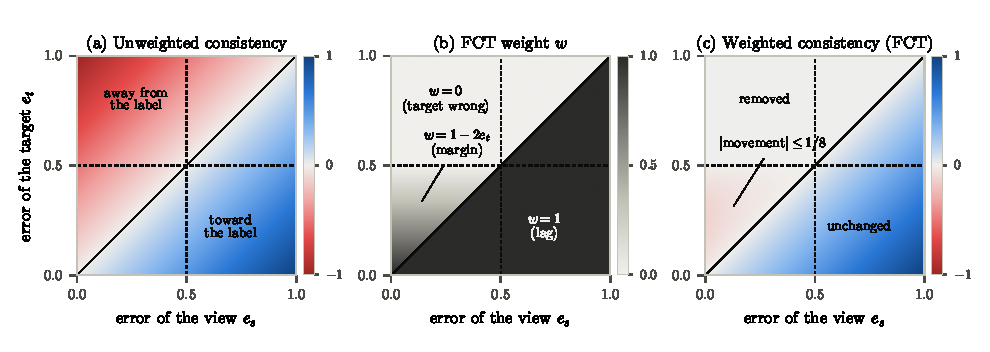
\includegraphics[width=0.96\textwidth]{figures/fig_pull.pdf}
\caption{Effect of a consistency term on the error of a view at one pixel, as a function of the view's
error $e_s$ and the error $e_t$ of its detached target (Proposition~\ref{prop:identity}); dashed lines
mark the decision threshold. (a)~Without a weight, the term moves the view away from the label wherever
the view is the closer of the two, even toward a wrong target (top left). (b)~The FCT weight of
Eq.~\eqref{eq:weight}. (c)~With it, every movement toward the label is kept, every movement away from
the label toward a wrong target is removed, and the remaining movements away from the label are
bounded by $1/8$.}
\label{fig:pull}
\end{figure*}

In semi-supervised learning, no label separates the two cases, so the views are drawn together alike.
Under full supervision, the label separates them at every pixel: the term can keep its full weight
where the view lags behind its target, and elsewhere act only where it cannot reverse a correct
decision. Section~\ref{sec:method} turns this rule into the weights of the FCT loss.

\section{Flip-Consistent Training}
\label{sec:method}

FCT is a training loss. It replaces the supervised loss of a segmentation network with three parts:
the supervised loss on three orientation views of each image, a consistency term that draws the
predictions of the views together, and label-aware weights that decide, pixel by pixel, how much
each view may move toward another (Fig.~\ref{fig:overview}). The network and its inference are
unchanged. This section describes the three parts and the full loss, and then relates FCT to other
losses.

\begin{figure*}[t]
\centering
% Overview of FCT (Section IV). Needs \usepackage{tikz} and
% \usetikzlibrary{arrows.meta,positioning,calc,fit,backgrounds}.
% Thumbnails: figures/ov/*.png (a Kvasir-SEG training image, its two flips and its label).
\definecolor{flipc}{HTML}{2A78D6}
\definecolor{upc}{HTML}{EB6834}
\begin{tikzpicture}[
  font=\footnotesize, >={Stealth[length=4.2pt,width=3.8pt]},
  img/.style={inner sep=0pt, draw=black!35, line width=0.3pt},
  net/.style={draw=black!70, line width=0.5pt, fill=black!4, rounded corners=1.5pt,
              minimum width=9mm, minimum height=7mm, align=center},
  map/.style={draw=black!70, line width=0.5pt, fill=white, minimum width=8mm, minimum height=7mm},
  sup/.style={draw=black!60, line width=0.4pt, fill=black!4, rounded corners=1.5pt,
              minimum height=5.5mm, inner xsep=2.5pt, align=center},
  flow/.style={->, line width=0.5pt, black!75},
  pull/.style={->, line width=1.2pt},
  lab/.style={font=\scriptsize, black!85, align=center},
]
  \def\th{10.5mm}
  % ---- inputs: the image and its two flips -------------------------------------
  \node[img] (xh) at (0, 1.45)  {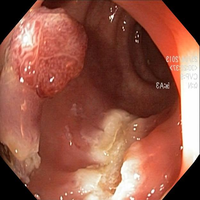
\includegraphics[width=\th]{figures/ov/xh.png}};
  \node[img] (x)  at (0, 0)     {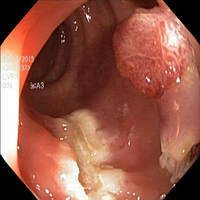
\includegraphics[width=\th]{figures/ov/x.png}};
  \node[img] (xv) at (0, -1.45) {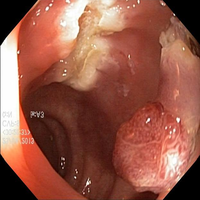
\includegraphics[width=\th]{figures/ov/xv.png}};
  \node[lab, left=1.2mm of xh] {$T_h x$};
  \node[lab, left=1.2mm of x]  {$x$};
  \node[lab, left=1.2mm of xv] {$T_v x$};
  % ---- one network, three passes ------------------------------------------------
  \node[net] (fh) at (1.6, 1.45)  {$f$};
  \node[net] (fo) at (1.6, 0)     {$f$};
  \node[net] (fv) at (1.6, -1.45) {$f$};
  \draw[flow] (xh) -- (fh); \draw[flow] (x) -- (fo); \draw[flow] (xv) -- (fv);
  \begin{scope}[on background layer]
    \node[draw=black!35, dashed, line width=0.4pt, rounded corners=2pt, fit=(fh)(fv), inner sep=2.2mm] (shared) {};
  \end{scope}
  \node[lab, below=0.6mm of shared] {shared weights,\\ same depth mask};
  % ---- logits in the upright frame -----------------------------------------------
  \node[map] (zh) at (3.45, 1.45)  {$z^{h}$};
  \node[map] (zo) at (3.45, 0)     {$z^{o}$};
  \node[map] (zv) at (3.45, -1.45) {$z^{v}$};
  \draw[flow] (fh) -- node[lab, above, pos=0.62] {$T_h^{-1}$} (zh);
  \draw[flow] (fo) -- (zo);
  \draw[flow] (fv) -- node[lab, above, pos=0.62] {$T_v^{-1}$} (zv);
  % ---- (1) the three supervised views ---------------------------------------------
  \node[sup] (sh) at (5.2, 1.45)  {$\tfrac13\mathcal{L}_{\mathrm{host}}$};
  \node[sup] (so) at (5.2, 0)     {$\tfrac13\mathcal{L}_{\mathrm{host}}$};
  \node[sup] (sv) at (5.2, -1.45) {$\tfrac13\mathcal{L}_{\mathrm{host}}$};
  \draw[flow] (zh) -- (sh); \draw[flow] (zo) -- (so); \draw[flow] (zv) -- (sv);
  \node[img] (y) at (6.85, 0) {
\includegraphics[width=\th]{figures/ov/y.png}};
  \node[lab, below=0.6mm of y] {label $y$};
  \draw[flow, black!45] (y.north west) -- (sh.east);
  \draw[flow, black!45] (y.west) -- (so.east);
  \draw[flow, black!45] (y.south west) -- (sv.east);
  \node[lab, above=1.4mm of sh, xshift=4mm] {(1) three supervised views};
  % ---- (2) the consistency term between the views' probabilities -----------------
  \node[map] (po) at (8.75, 0)     {$p^{o}$};
  \node[map] (ph) at (10.95, 1.15) {$p^{h}$};
  \node[map] (pv) at (10.95, -1.15) {$p^{v}$};
  \draw[pull, flipc] (po.north) to[bend left=28] node[lab, above left, pos=0.45, xshift=1mm] {$C_h$, weight $w_h$} (ph.west);
  \draw[pull, upc]   (ph.south) to[bend left=28] (po.east);
  \draw[pull, flipc] (po.south) to[bend right=28] node[lab, below left, pos=0.45, xshift=1mm] {$C_v$, weight $w_v$} (pv.west);
  \draw[pull, upc]   (pv.north) to[bend right=28] (po.east);
  \node[lab] at (9.95, 0.47) {$U$, gate $g$};
  \node[lab] at (9.85, 2.25) {(2) label-aware consistency, $p=\sigma(z)$};
  \node[lab, anchor=west] at (11.55, 0.35) {\textcolor{flipc}{\rule[0.5ex]{3mm}{1.2pt}} flipped views:};
  \node[lab, anchor=west] at (11.55, 0.0) {lag or margin};
  \node[lab, anchor=west] at (11.55, -0.45) {\textcolor{upc}{\rule[0.5ex]{3mm}{1.2pt}} upright view:};
  \node[lab, anchor=west] at (11.55, -0.8) {best flip, gated};
  \node[lab] at (9.85, -2.2) {arrow: detached target $\to$ view it moves};
\end{tikzpicture}

\caption{Overview of the FCT loss. (1)~An image and its horizontal and vertical flips pass through one
network; the flipped outputs are flipped back, and each view is supervised with the host network's own
loss, weighted $\frac13$. (2)~A consistency term draws the predictions of the views together, each
toward a detached target: the flipped views toward the upright view, with the lag-or-margin weight of
Eq.~\eqref{eq:weight}, and the upright view toward the flipped view closest to the label, wherever that
view is more accurate. At test time, only the upright view is used.}
\label{fig:overview}
\end{figure*}

\subsection{Multi-View Supervision}
\label{sec:views}

Each image is passed through the network upright and flipped horizontally and vertically, and the
flipped outputs are flipped back to the upright frame as in Eq.~\eqref{eq:views}. Every view is
supervised with the host network's own loss:
\begin{equation}
\mathcal{L}_{\mathrm{sup}}=\frac13\sum_{k\in\{o,h,v\}}\mathcal{L}_{\mathrm{host}}\big(Z^{k},y\big),
\label{eq:sup}
\end{equation}
where $Z^{k}$ denotes all output maps of view $k$ in the upright frame and $\mathcal{L}_{\mathrm{host}}$
the supervised loss of the host network, unchanged; the prediction logit $z^{k}$ is formed from $Z^{k}$
as the host forms it at test time. The factor $\frac13$ keeps the supervised loss at the scale of
single-view training. On its own, Eq.~\eqref{eq:sup} is a deterministic form of flip augmentation:
each view is tied to the label, but no view is tied to another.

\subsection{Cross-View Consistency}
\label{sec:flippull}

The consistency term ties the views to each other. It draws each flipped view $k$ toward the detached
upright prediction,
\begin{equation}
\mathcal{C}_k=\frac{1}{HW}\sum_{i} w^{k}_i\,\ell\big(z^{k}_i;p^{o}_i\big),
\label{eq:flippull}
\end{equation}
with the weights $w^{k}_i$ of Section~\ref{sec:weights}, and it draws the upright view toward the flipped
view closest to the label, wherever that view is more accurate:
\begin{equation}
\mathcal{U}=\frac{1}{HW}\sum_{i} g_i\,\ell\big(z^{o}_i;p^{\ast}_i\big),\qquad g_i=\mathbf{1}\big[e^{\ast}_i<e^{o}_i\big],
\label{eq:uppull}
\end{equation}
where $p^{\ast}_i$ denotes the detached probability of the flipped view with the smaller error at
pixel $i$, and $e^{\ast}_i$ its error. Together, the two directions let the more accurate side move the
other: where the upright view is more accurate, the flipped views move toward it, and where a flipped
view is more accurate, the upright view, which is the one used at test time, moves toward it. By
Corollary~\ref{cor:lag}, every movement that the gate $g$ allows in Eq.~\eqref{eq:uppull} is toward the
label.

\subsection{Label-Aware Weights}
\label{sec:weights}

The weights decide how much each flipped view moves toward the upright view. Following
Corollary~\ref{cor:lag}, the term keeps its full weight where the flipped view lags behind the upright
view, and it is weakened where the flipped view leads:
\begin{equation}
w^{k}_i=\begin{cases}1, & e^{k}_i\geq e^{o}_i,\\ \max\big(0,\,1-a\,e^{o}_i\big), & e^{k}_i<e^{o}_i,\end{cases}
\label{eq:weight}
\end{equation}
where $e^{k}_i$ and $e^{o}_i$ denote the errors of the flipped and the upright view at pixel $i$, computed
without gradient, and $a>0$ is a constant.

The constant $a$ follows from the decision threshold. On a leading pixel, the term moves the flipped
view away from the label (Corollary~\ref{cor:lag}), and Eq.~\eqref{eq:weight} keeps it in proportion to
the margin $1-a\,e^{o}$. We ask two things of this margin. First, a movement toward a wrong target must
vanish, $w=0$ whenever $e^{o}>\frac12$, which requires $a\geq2$. Second, a movement toward a correct
target must survive however small its margin, $w>0$ whenever $e^{o}<\frac12$, which requires
$a\leq2$. Hence $a=2$, and on a leading pixel with a correct target, $w=1-2e^{o}=|2p^{o}-1|$ is twice
the target's distance from the threshold, that is, its margin rescaled to $[0,1]$. The constant is thus
set by the threshold rather than tuned, and Section~\ref{sec:ablation} shows that the results are
insensitive to it.

With $a=2$, the term on a leading pixel is weak. Its strength $w\,(e^{o}-e^{k})$ is at most
$(1-2e^{o})\,e^{o}\leq\frac18$, against up to one for a supervised step (Fig.~\ref{fig:pull}(c)), and it
vanishes when the flipped view reaches the upright prediction, on the correct side of the threshold. It
thus keeps the two views consistent where both are right, as flip equivariance asks, without reversing a
decision by itself.

\subsection{Full Loss and Training}
\label{sec:objective}

The FCT loss adds the consistency term to the multi-view supervision:
\begin{equation}
\mathcal{L}_{\mathrm{FCT}}=\mathcal{L}_{\mathrm{sup}}+\frac{\lambda}{2}\big(\mathcal{C}_h+\mathcal{C}_v\big)+\frac{\lambda}{2}\,\mathcal{U},
\label{eq:objective}
\end{equation}
where $\lambda\geq0$ weighs consistency against supervision. The two flipped views share $\lambda$, and
the upright view's term receives the weight of one flipped view's. The weight is ramped up linearly at
the start of training,
\begin{equation}
\lambda_t=\lambda\,\min\big(1,\,t/t_0\big),
\label{eq:ramp}
\end{equation}
where $t$ counts the training batches and $t_0$ is the length of the ramp; we use $\lambda=0.5$ and
$t_0=300$.

Three implementation choices keep the views comparable and the memory low. First, the three views of
an image share one stochastic-depth mask~\cite{huang2016stochastic}, so that their differences reflect
the flip rather than the random depth. Second, when a host trains at several input scales, FCT is
applied at every scale. Third, the probabilities $p^{h}$ and $p^{v}$ of Eq.~\eqref{eq:uppull} come from
passes without gradient that leave the running statistics of batch normalization unchanged. In our
current implementation, these passes run before the upright pass and the graph of each view is
released after its backward pass, so only one view's computation graph is held in memory at a time;
the runs reported in Section~\ref{sec:experiments} computed them after the upright pass, which gives
the same loss at a higher peak memory. For each image and input scale, FCT thus runs five forward
passes, three of them with gradients. At test time, the network is applied to the upright image only,
exactly as without FCT, so FCT changes neither the architecture nor its inference cost.

\subsection{Relation to Other Losses}
\label{sec:relation}

By Eq.~\eqref{eq:combined}, FCT is a supervised loss with adaptive pixel weights: on a flipped view,
the supervised weight $\frac13$ is raised where the view lags behind the upright view and slightly
lowered where it leads. This places FCT among losses that reweight pixels. Focal
loss~\cite{lin2017focal} and online hard example mining~\cite{shrivastava2016ohem} weight a pixel by its
own error, and the structure loss of PraNet-style networks~\cite{wei2020f3net} by its distance to a
boundary; FCT weights it by how its error compares with that of another view of the same pixel.

The weights of Eq.~\eqref{eq:weight} also contain the usual consistency rules as special cases or near
neighbours, which Section~\ref{sec:ablation} compares. With $w=1$ everywhere, $\mathcal{C}_k$ is the
unweighted transformation consistency of semi-supervised
segmentation~\cite{bortsova2019consistency,li2021tcsm}, applied here to labeled images; by
Eq.~\eqref{eq:weights}, it mixes positive and negative pixel weights. Confidence
thresholding~\cite{sohn2020fixmatch} keeps the terms whose target is confident, which includes
confidently wrong targets, the case that Corollary~\ref{cor:lag} rules out. Finally, a rule can use the
label to judge the target alone, for example by weighting each pixel by whether and how confidently the
upright view is correct. Such a rule ignores the error of the view being moved, so it cannot tell the
lagging pixels, where the term helps, from the leading ones, where it hurts. Of these rules, only FCT
compares the two errors, as Corollary~\ref{cor:lag} requires.

\section{Experiments}
\label{sec:experiments}

We test the claims of Sections~\ref{sec:analysis} and~\ref{sec:method} in the order in which they were
made: FCT improves all three networks over their own baselines, most on
unseen data (Section~\ref{sec:main}), and a label-aware variant generalizes to six more centres
(Section~\ref{sec:polypgen}); FCT makes predictions more flip-consistent
(Section~\ref{sec:flip}); a per-image analysis shows where its gains come from
(Section~\ref{sec:where}); and a study of the loss terms shows that the multi-view supervision gives
most of the gain, while the label-aware weights shape the gradient as Corollary~\ref{cor:lag} predicts and
need no tuning (Section~\ref{sec:ablation}).
Section~\ref{sec:cost} reports its cost.

\subsection{Datasets and Evaluation Protocol}
\label{sec:setup}

We train on 1,288 images, 800 from Kvasir-SEG~\cite{jha2020kvasir} and 488 from
CVC-ClinicDB~\cite{bernal2015clinicdb}, drawn from the 1,450-image training split
of~\cite{fan2020pranet}; none of them appears in a test set. Because this set is smaller than the full
split, absolute scores are not directly comparable with published ones, and every comparison below is
between models trained on the same images. We test on the five standard test sets: the test splits of
Kvasir-SEG (100 images) and CVC-ClinicDB (62), which we call seen, and
CVC-ColonDB~\cite{tajbakhsh2016colondb} (380), CVC-300~\cite{vazquez2017endoscene} (60) and
ETIS~\cite{silva2014etis} (196), which are unseen in training. CVC-ColonDB and CVC-300 come from the same
group as CVC-ClinicDB, whereas ETIS comes from another centre.

We report the mean Dice (mDice) of the evaluation toolbox of~\cite{fan2020pranet}, which Polyp-PVT also
uses: each predicted map is min-max normalized and binarized at 256 thresholds, and the Dice coefficient
is averaged over images and thresholds. The flip gap of Eq.~\eqref{eq:flipgap} is computed on the masks
thresholded at 0.5 at the input resolution of the network, with add-one smoothing so that two empty
masks agree. Each network is evaluated on the five test sets after every epoch with the per-image Dice
of the official Polyp-PVT code, and we keep the epoch with the highest five-set mean, for vanilla and
FCT alike; Section~\ref{sec:main} also reports the gains without this selection.

Each configuration is trained with six random seeds, and vanilla and FCT share each seed. We report
the mean and standard deviation (SD) over seeds, the mean paired difference with its 95\% confidence
interval (CI) from the $t$-distribution with five degrees of freedom, and the number of seeds on which
FCT scores higher. An exact permutation test over all 924 ways of splitting the twelve runs of a
comparison into two groups of six reaches the same conclusion as the CI for every entry of
Tables~\ref{tab:main_polyppvt} and~\ref{tab:main_pranetv2}.

\subsection{Implementation Details}
\label{sec:implementation}

We add FCT to three networks without changing their architectures or retuning their recipes.
Polyp-PVT~\cite{dong2023polyppvt} uses a PVTv2-B2 encoder~\cite{wang2022pvtv2}. As in its official code,
it is trained with AdamW, a learning rate of $10^{-4}$, a weight decay of $10^{-4}$, batches of 16 images
of $352\times352$ pixels, input scales of 0.75, 1 and 1.25, element-wise gradient clipping at 0.5 and 99 epochs, and
its encoder has a stochastic-depth rate of 0.1; we add mixed precision. Its official recipe applies no orientation
augmentation by default, and we keep this default, so vanilla Polyp-PVT never sees a flipped image.
PraNet-V2~\cite{hu2026pranetv2} uses a Res2Net-50 encoder~\cite{gao2021res2net}, which has no stochastic
depth, and is trained with Adam, a constant learning rate of $10^{-4}$, batches of 8 images and 29
epochs, with the data pipeline, input scales and mixed precision of Polyp-PVT. ASGNet~\cite{sun2026asgnet} uses a PVTv2-B3 encoder and keeps its own
recipe: Adam, batches of 40 images accumulated over eight parts, 79 epochs at a single scale in full
precision, a cosine learning-rate schedule, and its own data loader, which applies random horizontal
flips, crops, rotations, colour changes and label noise. Unlike the other two, ASGNet is therefore
trained with flip augmentation even without FCT. FCT uses $\lambda=0.5$, set in preliminary runs on
Polyp-PVT, and $a=2$ for all three networks. Each run uses one \pend{[GPU model]} GPU.

\subsection{Main Results}
\label{sec:main}

FCT improves the five-set mean Dice of Polyp-PVT and PraNet-V2 on every seed and that of ASGNet on
five of six, and for every network its largest gain is on an unseen set
(Tables~\ref{tab:main_polyppvt}--\ref{tab:main_asgnet}, Fig.~\ref{fig:seeds}). For
Polyp-PVT, the five-set mean rises by 0.52 points, with a 95\% CI of $[0.15, 0.90]$, and ETIS gains 1.65
points $[0.88, 2.42]$ on all six seeds; the gains on the other four sets are positive on average but
within seed variation. For PraNet-V2, the five-set mean rises by 1.68 points $[0.69, 2.67]$. Its largest
gains are on ETIS, 3.61 points $[0.23, 6.99]$, and on CVC-ColonDB, 3.01 points $[1.25, 4.77]$ on all six
seeds, and Kvasir also improves, by 1.69 points $[0.12, 3.26]$. For PraNet-V2, FCT also lowers the SD over
seeds on every set. For these two networks, no set loses on average; the smallest gains are on
CVC-300 for both, $+0.06$ and $+0.04$ points, and on CVC-ClinicDB for PraNet-V2, $+0.03$. ASGNet, whose
own recipe already trains with random horizontal flips, gains least (Table~\ref{tab:main_asgnet}).
Its ETIS score rises by 1.69 points $[0.08, 3.30]$ on five of six seeds, but its five-set mean rises by
only 0.31 points: the CI excludes zero by less than 0.01 points (paired $p=0.049$), and the exact
permutation test does not support the gain ($p=0.20$). Its other four sets change by less than 0.6
points in either direction, within seed variation.

% Generated by make_table.py from seeds_s3lmup.out (S3LMUP vs PVT_VANILLA); do not edit by hand.
\begin{table}[t]
\centering
\footnotesize
\setlength{\tabcolsep}{2.6pt}
\begin{threeparttable}
\caption{Polyp-PVT (PVTv2-B2) with and without FCT on five polyp test sets: mDice (\%), mean $\pm$ SD over six seeds. Bold: gains whose 95\% CI excludes zero.}
\label{tab:main_polyppvt}
\begin{tabular}{@{}l r@{$\,\pm\,$}l r@{$\,\pm\,$}l r r@{, }l c@{}}
\toprule
Test set & \multicolumn{2}{c}{Vanilla} & \multicolumn{2}{c}{FCT (ours)} & Gain & \multicolumn{2}{c}{95\% CI} & Seeds \\
\midrule
\multicolumn{9}{@{}l}{\textit{Seen}} \\
\enspace Kvasir & 91.94 & 0.59 & 92.50 & 0.41 & +0.56 & [$-$0.31 & 1.44] & 4/6 \\
\enspace CVC-ClinicDB & 93.17 & 0.64 & 93.36 & 0.23 & +0.19 & [$-$0.64 & 1.01] & 4/6 \\
\addlinespace[2pt]
\multicolumn{9}{@{}l}{\textit{Unseen}} \\
\enspace CVC-ColonDB & 80.28 & 0.68 & 80.43 & 0.60 & +0.15 & [$-$0.80 & 1.10] & 3/6 \\
\enspace CVC-300 & 88.79 & 0.86 & 88.85 & 1.10 & +0.06 & [$-$1.39 & 1.51] & 2/6 \\
\enspace ETIS & 78.61 & 0.29 & 80.26 & 0.65 & \textbf{+1.65} & \textbf{[0.88} & \textbf{2.42]} & 6/6 \\
\midrule
Mean & 86.56 & 0.17 & 87.08 & 0.32 & \textbf{+0.52} & \textbf{[0.15} & \textbf{0.90]} & 6/6 \\
\bottomrule
\end{tabular}
\begin{tablenotes}[flushleft]
\footnotesize
\item Training set: 1,288 Kvasir and \mbox{CVC-ClinicDB} images; \textit{seen}: test splits of the two training datasets; \textit{unseen}: datasets not used in training. Gain: mean paired difference, FCT minus vanilla with the same seed. 95\% CI: $t$-distribution, five degrees of freedom. Seeds: seeds, of six, on which FCT scores higher. Mean: average over the five test sets.
\end{tablenotes}
\end{threeparttable}
\end{table}

% Generated by make_table.py from seeds_pranetv2.out (PRANETV2_S3LMUP vs PRANETV2_VANILLA); do not edit by hand.
\begin{table}[t]
\centering
\footnotesize
\setlength{\tabcolsep}{2.6pt}
\begin{threeparttable}
\caption{PraNet-V2 (Res2Net-50) with and without FCT on five polyp test sets: mDice (\%), mean $\pm$ SD over six seeds. Bold: gains whose 95\% CI excludes zero.}
\label{tab:main_pranetv2}
\begin{tabular}{@{}l r@{$\,\pm\,$}l r@{$\,\pm\,$}l r r@{, }l c@{}}
\toprule
Test set & \multicolumn{2}{c}{Vanilla} & \multicolumn{2}{c}{FCT (ours)} & Gain & \multicolumn{2}{c}{95\% CI} & Seeds \\
\midrule
\multicolumn{9}{@{}l}{\textit{Seen}} \\
\enspace Kvasir & 87.94 & 1.46 & 89.63 & 0.55 & \textbf{+1.69} & \textbf{[0.12} & \textbf{3.26]} & 5/6 \\
\enspace CVC-ClinicDB & 89.80 & 1.30 & 89.83 & 0.86 & +0.03 & [$-$1.31 & 1.38] & 3/6 \\
\addlinespace[2pt]
\multicolumn{9}{@{}l}{\textit{Unseen}} \\
\enspace CVC-ColonDB & 69.91 & 2.30 & 72.92 & 1.27 & \textbf{+3.01} & \textbf{[1.25} & \textbf{4.77]} & 6/6 \\
\enspace CVC-300 & 87.73 & 2.92 & 87.76 & 1.47 & +0.04 & [$-$3.31 & 3.39] & 3/6 \\
\enspace ETIS & 67.07 & 1.72 & 70.68 & 1.69 & \textbf{+3.61} & \textbf{[0.23} & \textbf{6.99]} & 5/6 \\
\midrule
Mean & 80.49 & 0.93 & 82.17 & 0.64 & \textbf{+1.68} & \textbf{[0.69} & \textbf{2.67]} & 6/6 \\
\bottomrule
\end{tabular}
\begin{tablenotes}[flushleft]
\footnotesize
\item Columns and statistics as in Table~\ref{tab:main_polyppvt}.
\end{tablenotes}
\end{threeparttable}
\end{table}

% Placeholder until ASGNet's six seeds finish. Regenerate it then with make_table.py (command in main.tex);
% the label stays the same, so the references in the text need no change.
\begin{table}[t]
\centering
\footnotesize
\begin{threeparttable}
\caption{ASGNet (PVTv2-B3) with and without FCT on five polyp test sets: mDice (\%), mean $\pm$ SD over six seeds. Bold: gains whose 95\% CI excludes zero.}
\label{tab:main_asgnet}
\begin{tabular}{@{}c@{}}
\toprule
\pend{Pending: the six ASGNet seeds are still training.} \\
\bottomrule
\end{tabular}
\end{threeparttable}
\end{table}


\begin{figure}[t]
\centering
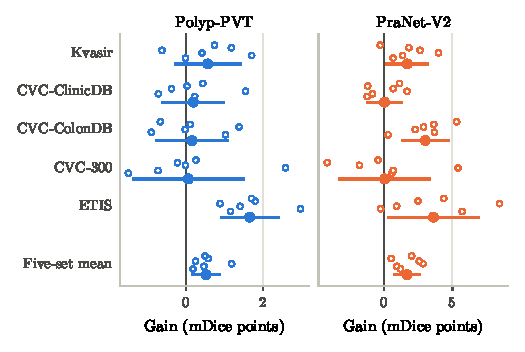
\includegraphics[width=\columnwidth]{figures/fig_seeds.pdf}
\caption{Paired gains of FCT over vanilla in mDice points: one hollow marker per seed, and the mean
with its 95\% CI below them. Every seed gains on the five-set mean for Polyp-PVT and PraNet-V2 and five
of six for ASGNet; the largest gains are on ETIS and, for PraNet-V2, CVC-ColonDB.}
\label{fig:seeds}
\end{figure}

Without epoch selection, the gains remain positive on average but are less certain.
Fig.~\ref{fig:curves} shows the five-set mean of the
training-time evaluator after every epoch: the six-seed mean of FCT lies above that of vanilla after 81
of 99 epochs for Polyp-PVT, 28 of 29 for PraNet-V2 and 76 of 79 for ASGNet. Averaged over the last ten
epochs, without any selection, FCT gains $+0.42$ $[-0.03, 0.88]$, $+2.41$ $[1.40, 3.43]$ and $+0.21$
$[-0.59, 1.01]$ points on the five-set mean of the three networks, and $+1.52$ $[0.11, 2.93]$, $+3.71$
$[0.75, 6.68]$ and $+1.99$ $[-0.26, 4.24]$ points on ETIS (Appendix, Table~\ref{tab:selfree}). At the last
epoch alone, no five-set mean gain has a CI above zero: $+0.55$ $[-0.11, 1.22]$ for Polyp-PVT, $+0.49$
$[-1.17, 2.14]$ for PraNet-V2, whose curves peak early and decline, so that its last epoch is a poor
checkpoint for either arm, and $+0.13$ $[-0.91, 1.17]$ for ASGNet.

\begin{figure}[t]
\centering
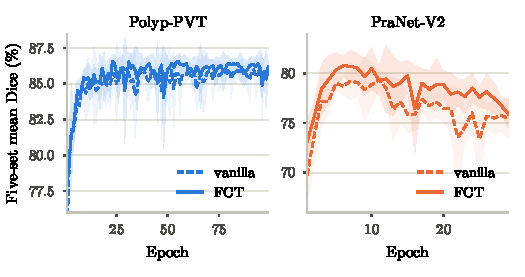
\includegraphics[width=\columnwidth]{figures/fig_curves.pdf}
\caption{Five-set mean Dice of the training-time evaluator after every epoch, without (dashed) and
with (solid) FCT; mean and SD over six seeds. FCT lies above vanilla through most of training. Every
ASGNet run, with or without FCT, drops briefly at epoch 62, so the drop comes from its recipe, not from
FCT.}
\label{fig:curves}
\end{figure}

\subsection{Six More Centres}
\label{sec:polypgen}

Of the five standard test sets, only ETIS comes from another centre than the training images
(Section~\ref{sec:setup}). PolypGen~\cite{ali2023polypgen} adds six more centres; we use its 1,411 single-frame images with a
polyp, none of which took part in training or in selecting a checkpoint. We fixed the analysis before
scoring any map: the primary result is the mDice pooled over the six centres, every image counted once,
over all six seeds, and each centre is a secondary result. So far, PolypGen maps exist only for the
confidence-graded weight, row (h) of Table~\ref{tab:rules}, and not yet for FCT. This label-aware
variant raises the pooled mDice of Polyp-PVT from 82.14\% to 82.98\%, by 0.84 points $[0.59, 1.09]$, on
all six seeds, and its gain has a CI above zero on four of the six centres (Table~\ref{tab:polypgen});
an exact permutation test over the 924 splits of the twelve runs gives $p=0.002$ for the pooled gain.
\pend{FCT's checkpoints will be scored with the same analysis.}

%% Generated by make_tables_extra.py; do not edit by hand.
\begin{table}[t]
\centering
\footnotesize
\setlength{\tabcolsep}{3pt}
\begin{threeparttable}
\caption{Six more centres (PolypGen): mDice (\%) of vanilla Polyp-PVT and of its confidence-graded variant, row (h) of Table~\ref{tab:rules}, mean $\pm$ SD over six seeds. Bold: gains whose 95\% CI excludes zero.}
\label{tab:polypgen}
\begin{tabular}{@{}l c c c c c@{}}
\toprule
Centre & Images & Vanilla & Variant (h) & Gain [95\% CI] & Seeds \\
\midrule
\enspace C1 & 251 & 86.65$\,\pm\,$0.42 & 87.94$\,\pm\,$0.55 & \textbf{+1.29 [0.71, 1.86]} & 6/6 \\
\enspace C2 & 270 & 84.60$\,\pm\,$0.47 & 84.31$\,\pm\,$0.64 & $-$0.28 [$-$1.27, 0.70] & 2/6 \\
\enspace C3 & 455 & 89.93$\,\pm\,$0.24 & 90.46$\,\pm\,$0.20 & \textbf{+0.53 [0.25, 0.81]} & 6/6 \\
\enspace C4 & 146 & 68.33$\,\pm\,$0.99 & 69.23$\,\pm\,$1.47 & +0.90 [$-$1.63, 3.44] & 4/6 \\
\enspace C5 & 206 & 65.71$\,\pm\,$1.65 & 67.92$\,\pm\,$1.25 & \textbf{+2.21 [0.38, 4.04]} & 5/6 \\
\enspace C6 & 83 & 82.88$\,\pm\,$0.29 & 84.23$\,\pm\,$0.45 & \textbf{+1.35 [1.04, 1.65]} & 6/6 \\
\midrule
Pooled & 1411 & 82.14$\,\pm\,$0.18 & 82.98$\,\pm\,$0.21 & \textbf{+0.84 [0.59, 1.09]} & 6/6 \\
\bottomrule
\end{tabular}
\begin{tablenotes}[flushleft]
\footnotesize
\item Single-frame images with a polyp; none was used in training or in selecting a checkpoint. Pooled: every image of the six centres counted once, the primary result of an analysis fixed before scoring. FCT itself: \pend{pending}.
\end{tablenotes}
\end{threeparttable}
\end{table}


\subsection{Flip Consistency}
\label{sec:flip}

FCT makes both networks more flip-consistent on every test set (Table~\ref{tab:flipgap}). It lowers the
five-set mean flip gap from 12.5\% to 7.5\% for Polyp-PVT and from 15.6\% to 10.2\% for PraNet-V2, and
the flip gap on the training images by 84\% and 76\%. The reduction holds on every seed and in every
row of the table. Two observations qualify it. First, flip consistency is not accuracy: the largest
reduction on a test set, 70\% for Polyp-PVT on CVC-ClinicDB, comes with almost no change in Dice, and CVC-ColonDB and
ETIS remain the least consistent sets after FCT. Second, training on flipped images lowers the flip
gap by itself. In preliminary single runs of Polyp-PVT, the multi-view supervision of row~(b) of
Table~\ref{tab:rules}, without the consistency term, reached a five-set flip gap of 8.2\%, and the official random flip and
rotation augmentation reached 6.8\%, below that of FCT; yet the five-set mean Dice of the latter,
85.75\%, was below that of every vanilla seed. A lower flip gap alone therefore does not explain the gains of FCT, and we
read it as a symptom that the views are tied together, not as the cause of the gains.

%% Generated by make_tables_extra.py; do not edit by hand.
\begin{table}[t]
\centering
\footnotesize
\setlength{\tabcolsep}{3.6pt}
\begin{threeparttable}
\caption{Flip gap (\%) of the predicted masks without and with FCT on each test set and on the training images, and its relative change. Means over six seeds; lower is better.}
\label{tab:flipgap}
\begin{tabular}{@{}l rrr rrr@{}}
\toprule
& \multicolumn{3}{c}{Polyp-PVT} & \multicolumn{3}{c}{PraNet-V2} \\
\cmidrule(lr){2-4} \cmidrule(l){5-7}
Images & Vanilla & FCT & Change & Vanilla & FCT & Change \\
\midrule
\multicolumn{7}{@{}l}{\textit{Seen}} \\
\enspace Kvasir & 6.3 & 4.1 & $-$35\% & 8.8 & 5.1 & $-$42\% \\
\enspace CVC-ClinicDB & 12.4 & 3.7 & $-$70\% & 13.1 & 5.9 & $-$55\% \\
\addlinespace[2pt]
\multicolumn{7}{@{}l}{\textit{Unseen}} \\
\enspace CVC-ColonDB & 16.9 & 11.3 & $-$33\% & 20.4 & 14.8 & $-$27\% \\
\enspace CVC-300 & 9.1 & 5.1 & $-$43\% & 9.8 & 6.2 & $-$37\% \\
\enspace ETIS & 17.8 & 13.2 & $-$26\% & 25.8 & 19.2 & $-$26\% \\
\midrule
Five-set mean & 12.5 & 7.5 & $-$40\% & 15.6 & 10.2 & $-$34\% \\
Training images & 6.3 & 1.0 & $-$84\% & 8.5 & 2.0 & $-$76\% \\
\bottomrule
\end{tabular}
\begin{tablenotes}[flushleft]
\footnotesize
\item Flip gap: one minus the Dice overlap of the binary masks predicted for an image and for its flipped copy, flipped back, averaged over horizontal and vertical flips and over images. FCT lowers it on every seed, in every row.
\end{tablenotes}
\end{threeparttable}
\end{table}


\subsection{Where Do the Gains Come From?}
\label{sec:where}

For PraNet-V2, the gains on the unseen sets are spread over many images: on ETIS, the 176 images
outside the ten largest gains and the ten largest losses contribute 2.94 of its 3.61 points. For
Polyp-PVT, they are more concentrated: on ETIS, the ten images with the largest gains contribute 1.78
points, more than the net gain of 1.65, and the other 176 images contribute 0.79.
Table~\ref{tab:errors} breaks the errors down at a threshold of 0.5 on the per-image min-max-normalized
maps. The two networks gain in different ways. PraNet-V2 fails less
often: the number of images with a Dice below 0.1 falls from 31.8 to 25.0 per run on ETIS and from 56.5
to 47.5 on CVC-ColonDB. Polyp-PVT fails about as often with FCT as without, 10.3 and 10.5 images per run
on ETIS; it gains instead by predicting less false-positive area, 1.31 instead of 1.52 times the polyp
area. In two cases, small polyps carry much of the gain:
the quarter of images with the smallest polyps gains 5.46 points on ETIS for Polyp-PVT and 6.16 points
on CVC-ColonDB for PraNet-V2. The pattern is not general: on ETIS, the smallest polyps gain 2.70 points
for PraNet-V2 and the next quarter 6.05, and on CVC-300 the smallest polyps lose with both networks. These
breakdowns are descriptive, and with four size groups per set and network, some differences are
expected by chance.

%% Generated by make_tables_extra.py; do not edit by hand.
\begin{table}[t]
\centering
\footnotesize
\setlength{\tabcolsep}{1.9pt}
\begin{threeparttable}
\caption{Where the gains come from on the unseen test sets, vanilla $\to$ FCT: failures, missed and false-positive area, and the gain on the smallest polyps. Means over six seeds.}
\label{tab:errors}
\begin{tabular}{@{}l c c c c c@{}}
\toprule
Test set & Gain & Failures & Missed area & False-pos.\ area & Smallest \\
\midrule
\multicolumn{6}{@{}l}{\textit{Polyp-PVT}} \\
\enspace CVC-ColonDB & +0.15 & 15.0 $\to$ 15.3 & 0.18 $\to$ 0.16 & 0.66 $\to$ 0.73 & $-$1.75 \\
\enspace CVC-300 & +0.06 & 0.2 $\to$ 0.0 & 0.06 $\to$ 0.06 & 0.23 $\to$ 0.27 & $-$2.38 \\
\enspace ETIS & +1.65 & 10.5 $\to$ 10.3 & 0.12 $\to$ 0.11 & 1.52 $\to$ 1.31 & +5.46 \\
\addlinespace[2pt]
\multicolumn{6}{@{}l}{\textit{PraNet-V2}} \\
\enspace CVC-ColonDB & +3.01 & 56.5 $\to$ 47.5 & 0.27 $\to$ 0.25 & 0.33 $\to$ 0.26 & +6.16 \\
\enspace CVC-300 & +0.04 & 0.2 $\to$ 0.0 & 0.05 $\to$ 0.06 & 0.25 $\to$ 0.23 & $-$1.85 \\
\enspace ETIS & +3.61 & 31.8 $\to$ 25.0 & 0.26 $\to$ 0.22 & 0.82 $\to$ 0.86 & +2.70 \\
\bottomrule
\end{tabular}
\begin{tablenotes}[flushleft]
\footnotesize
\item Gain: mDice points. Failures: images per run with Dice below 0.1 for the mask thresholded at 0.5 after per-image min-max normalization. Missed and false-positive area: at the same threshold, as fractions of the polyp area. Smallest: mDice gain on the quarter of the set with the smallest polyps.
\end{tablenotes}
\end{threeparttable}
\end{table}


Fig.~\ref{fig:qual} shows examples. Without FCT, PraNet-V2 misses the polyp in rows 1, 2 and 4, and
Polyp-PVT adds spurious regions in rows 1--3; with FCT, both predictions concentrate on the polyp. The last row shows the image on which FCT loses most: with FCT, Polyp-PVT adds a false region,
and PraNet-V2 misses the polyp.

\begin{figure*}[t]
\centering
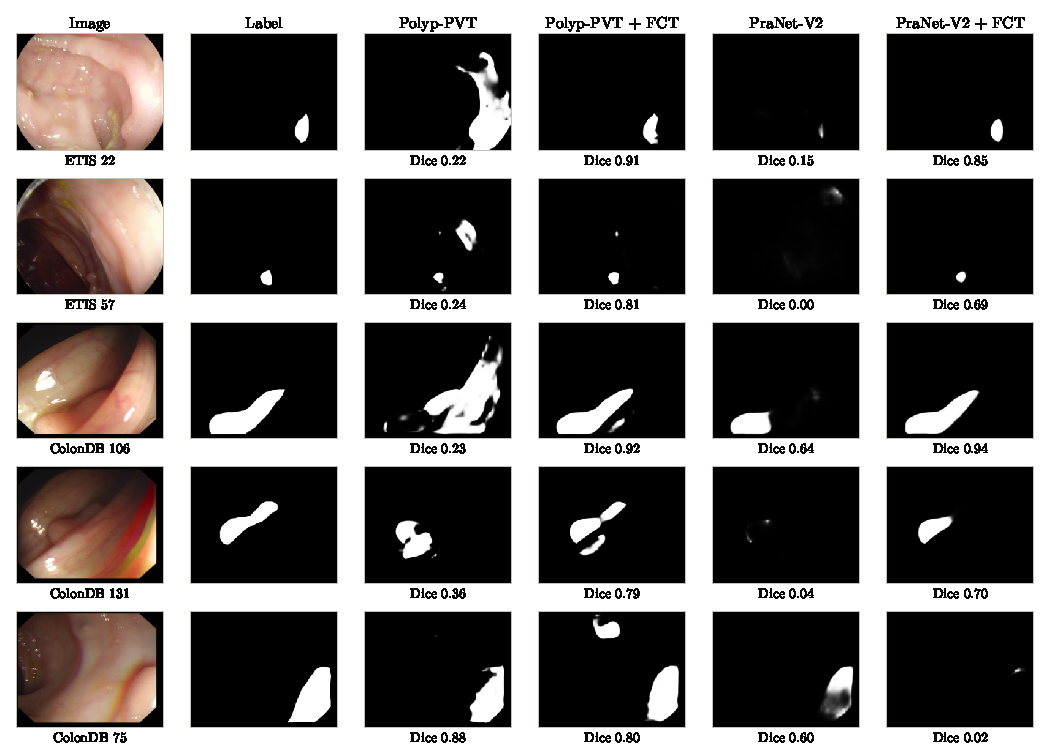
\includegraphics[width=0.94\textwidth]{figures/fig_qual.pdf}
\caption{Examples from the unseen sets: image, label, and the maps predicted by each network without
and with FCT (seed 1), each with its mDice. Rows 1--4: four of the twelve unseen-set images with the
largest gains, averaged over six seeds and both networks. Row 5: the image with the largest loss.}
\label{fig:qual}
\end{figure*}

\subsection{Ablation Studies}
\label{sec:ablation}

\textit{Loss terms.} The FCT loss has three parts: the multi-view supervision of Eq.~\eqref{eq:sup}, the
consistency term of Eqs.~\eqref{eq:flippull} and~\eqref{eq:uppull}, and the label-aware weights of
Eq.~\eqref{eq:weight}. Table~\ref{tab:rules} dissects them on Polyp-PVT, against the same vanilla runs
throughout. Row (b) keeps only the multi-view supervision. It is also the flip-augmentation control,
since it trains on exactly the views that FCT uses, with the same supervision. Rows (c)--(e) add the
consistency term on the upright view, on the flipped views, and on both, which is FCT, so their
differences from row (b) are the effect of the consistency term. Rows (f) and (g) change only the
weights of FCT, to unweighted consistency and to the lag gate without its margin. We fixed the protocol
before seeing these rows: rows (b) and (c) are trained with six seeds, and rows (f) and (g) with three
seeds first, extended to six only if they land near FCT. \pend{Row (c) is being repeated after a failed
run; rows (f) and (g) landed near FCT and are being extended to six seeds.} With six seeds, the paired
CI of the difference between two variants spans about $\pm0.4$ to $\pm0.7$ points on the five-set
mean, and with three seeds about 2.4 times more, so small differences between variants are not
resolved.

%% Generated by make_tables_extra.py; do not edit by hand.
\begin{table*}[t]
\centering
\footnotesize
\setlength{\tabcolsep}{2.6pt}
\begin{threeparttable}
\caption{Component dissection of FCT on Polyp-PVT: paired mDice gains (points, 95\% CI), the effect of each component, test sets improved, flip gap and gradient alignment. Bold: CIs that exclude zero.}
\label{tab:rules}
\begin{tabular}{@{}l c c c c c c c c c@{}}
\toprule
Variant & Views & Flip pulls & Upright pull & Mean gain & ETIS gain & Component effect & Sets & Flip gap (\%) & Cosine \\
\midrule
\multicolumn{10}{@{}l}{\textit{Building FCT on the three supervised views}} \\
(a) Vanilla & -- & -- & -- & -- & -- & -- & -- & 12.5 & -- \\
(b) Three views & \checkmark & -- & -- & \pend{pending} & \pend{pending} & -- & \pend{--} & \pend{--} & \pend{--} \\
(c) + upright pull & \checkmark & -- & \checkmark & \pend{pending} & \pend{pending} & \pend{pending} & \pend{--} & \pend{--} & \pend{--} \\
(d) + flip pulls & \checkmark & Eq.~\eqref{eq:weight} & -- & +0.47 [$-$0.02, 0.96] & \textbf{+1.97 [1.06, 2.87]} & \pend{pending} & 4/5 & 7.5 & 0.53 \\
(e) + both (FCT) & \checkmark & Eq.~\eqref{eq:weight} & \checkmark & \textbf{+0.52 [0.15, 0.90]} & \textbf{+1.65 [0.88, 2.42]} & \pend{pending} & 5/5 & 7.5 & 0.53 \\
\addlinespace[2pt]
\multicolumn{10}{@{}l}{\textit{Changing the weight function of FCT}} \\
(f) FCT, $w=1$ (3 seeds) & \checkmark & $w=1$ & \checkmark & \pend{pending} & \pend{pending} & \pend{pending} & \pend{--} & \pend{--} & \pend{--} \\
(g) FCT, lag only (3 seeds) & \checkmark & lag only & \checkmark & \pend{pending} & \pend{pending} & \pend{pending} & \pend{--} & \pend{--} & \pend{--} \\
\addlinespace[2pt]
\multicolumn{10}{@{}l}{\textit{Another label-aware weight, without the upright pull}} \\
(h) Graded weight & \checkmark & graded & -- & \textbf{+0.40 [0.13, 0.68]} & \textbf{+1.56 [0.53, 2.60]} & +0.06 [$-$0.60, 0.73] & 3/5 & 7.7 & 0.26 \\
\bottomrule
\end{tabular}
\begin{tablenotes}[flushleft]
\footnotesize
\item Six seeds unless the row says otherwise. Mean and ETIS gain: over vanilla with the same seeds. Component effect, on the five-set mean, paired by seed: for rows (c)--(e), the row minus row (b), so the effect of the pulls added to the three views; for rows (f) and (g), FCT minus the row, the effect of FCT\textquotesingle s weight function; for row (h), row (d) minus row (h). Sets: test sets, of five, with a positive mean gain. Cosine: between the gradient of the flip pulls and that of the rest of the objective, measured every 50 batches and averaged over training and seeds; for row (e), the rest includes the upright pull. Lag only: $w=1$ where the flipped view lags and $0$ where it leads ($a\to\infty$). Graded: the confidence-graded weight of Section~\ref{sec:ablation}.
\end{tablenotes}
\end{threeparttable}
\end{table*}


The multi-view supervision gives most of the gain on ETIS. On its own, row (b) raises ETIS by 1.48
points $[0.32, 2.65]$ on five of six seeds, against 1.65 points for FCT, and the five-set mean by 0.37
points $[-0.01, 0.74]$. This gain is not that of random flip augmentation: ASGNet already trains with
random flips, and FCT still raises its ETIS score by 1.69 points (Table~\ref{tab:main_asgnet}). The consistency term and its weights complete the loss: FCT is the only
variant that improves all five sets on average. The multi-view supervision alone lowers CVC-ClinicDB
by 0.48 points, and FCT recovers it, although this difference is borderline, $+0.66$ $[-0.01, 1.34]$.
The consistency term's own effect on the five-set mean, row (e) minus row (b), is $+0.16$
$[-0.30, 0.62]$ points, and the weight functions are within seed variation of one another: FCT minus
rows (f) and (g) is $+0.29$ $[-0.87, 1.45]$ and $+0.29$ $[-1.65, 2.23]$ points on three seeds, and
row (d) minus row (h) is $+0.06$ $[-0.60, 0.73]$. Row (h) uses the confidence-graded weight sketched in
Section~\ref{sec:relation}, which keeps a weight of 1 where the upright view is correct, raises it to
$1+p^{o}$ on missed polyp pixels and lowers it to $1-p^{o}$ on false-positive pixels.

The weights shape the gradient of the consistency term, as Eq.~\eqref{eq:weights} predicts. With the
lag-based weights of rows (d), (e) and (g), the gradient of the term on the flipped views has a cosine
of 0.53 to 0.56 with the gradient of the rest of the loss, and between 0.47 and 0.56 on every seed.
Without weights, row (f), it falls to 0.23, and with the confidence-graded weight, row (h), to 0.26;
these two stay between 0.18 and 0.33 on every seed (Fig.~\ref{fig:cos}). Unweighted and
confidence-graded terms keep full weight on leading flipped views, whose pixel weights in
Eq.~\eqref{eq:weights} are negative, so part of their gradient points away from the label. Leading
pixels are common: in the runs where we logged them, Polyp-PVT with $a<2$ and PraNet-V2, a flipped view
leads the upright view on about 44\% of its pixels at the end of training, although this is a share of
pixels, not of the gradient. The ratio of the two gradients' norms follows the same order: 0.07 to 0.08
with lag-based weights, against 0.11 without weights and 0.12 with the graded weight.

\begin{figure}[t]
\centering
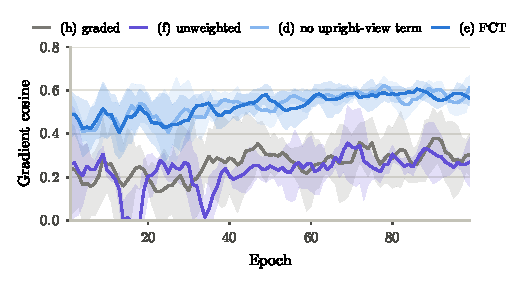
\includegraphics[width=\columnwidth]{figures/fig_cos.pdf}
\caption{Cosine between the gradient of the consistency term on the flipped views and that of the rest
of the loss during training of Polyp-PVT, for rows (d), (e), (f) and (h) of Table~\ref{tab:rules};
per-epoch means, smoothed over five epochs, with the SD over seeds. The lag-based weights double the
alignment of the consistency gradient with the rest of the loss.}
\label{fig:cos}
\end{figure}

\textit{Constant $a$.} The results are insensitive to $a$, so the constant needs no tuning
(Table~\ref{tab:sweep}; row (g) of Table~\ref{tab:rules} adds the limit $a\to\infty$, which keeps only
the lagging terms). Every value in $\{0.5, 1, 1.5, 2\}$ improves ETIS by 1.6 to 2.1 points, and none
differs significantly from $a=2$ on the five-set mean. The value $a=2$ is the only one that improves all
five sets on average, but this distinction is within seed variation. These runs do not fully explain
the insensitivity. The case that $a=2$ removes, a flipped view that leads a wrong upright view, is rare: it
arises on only 0.16\% of the pixels at the end of training (Polyp-PVT, $a<2$) and on 0.24\% (PraNet-V2).
But $a$ also scales the term on the far more frequent leading pixels with a correct upright view, and
this change, too, leaves Dice unchanged within seed variation.

%% Generated by make_tables_extra.py; do not edit by hand.
\begin{table}[t]
\centering
\footnotesize
\setlength{\tabcolsep}{2.2pt}
\begin{threeparttable}
\caption{Sensitivity to the constant $a$ of Eq.~\eqref{eq:weight} on Polyp-PVT: paired mDice gains over vanilla and over $a=2$ (points, six seeds, 95\% CI). Bold: CIs that exclude zero.}
\label{tab:sweep}
\begin{tabular}{@{}l c c c c@{}}
\toprule
$a$ & Mean gain & ETIS gain & Sets & $a=2$ minus row \\
\midrule
0.5 & \textbf{+0.51 [0.30, 0.73]} & \textbf{+2.15 [1.37, 2.92]} & 3/5 & +0.01 [$-$0.47, 0.49] \\
1 & +0.33 [$-$0.02, 0.67] & \textbf{+1.58 [0.40, 2.77]} & 3/5 & +0.19 [$-$0.26, 0.65] \\
1.5 & \textbf{+0.36 [0.02, 0.71]} & \textbf{+1.83 [0.83, 2.82]} & 3/5 & +0.16 [$-$0.24, 0.56] \\
2 (FCT) & \textbf{+0.52 [0.15, 0.90]} & \textbf{+1.65 [0.88, 2.42]} & 5/5 & -- \\
\bottomrule
\end{tabular}
\begin{tablenotes}[flushleft]
\footnotesize
\item Gains over vanilla on the five-set mean and on ETIS. Sets: test sets, of five, with a positive mean gain. Last column: paired difference on the five-set mean between $a=2$ and the row.
\end{tablenotes}
\end{threeparttable}
\end{table}


\subsection{Cost}
\label{sec:cost}

FCT multiplies the training time per epoch by 3.6 for Polyp-PVT, 3.3 for PraNet-V2 and 3.7 for ASGNet
(Table~\ref{tab:cost}). This matches its five forward and three backward passes for each image and input scale,
which cost $11/3\approx3.7$ times a single view if a backward pass costs twice a forward pass. Without
the term on the upright view, the two passes without gradient are not needed, and the measured factor
drops to 3.0. Inference
is unchanged: the trained network is the host network, applied once to the upright image.

%% Generated by make_tables_extra.py; do not edit by hand.
\begin{table}[t]
\centering
\footnotesize
\begin{threeparttable}
\caption{Cost of FCT: training time per epoch (minutes, median over six seeds) and inference cost.}
\label{tab:cost}
\begin{tabular}{@{}l c c c c@{}}
\toprule
Network & Vanilla & FCT & Ratio & Inference \\
\midrule
Polyp-PVT & 0.56 & 2.01 & 3.6$\times$ & unchanged \\
PraNet-V2 & 0.93 & 3.11 & 3.3$\times$ & unchanged \\
ASGNet & 1.01 & 3.70 & 3.7$\times$ & unchanged \\
Polyp-PVT, no upright-view term & 0.56 & 1.67 & 3.0$\times$ & unchanged \\
\bottomrule
\end{tabular}
\begin{tablenotes}[flushleft]
\footnotesize
\item Training time excludes the per-epoch evaluation. One \pend{[GPU model]} GPU per run. No upright-view term: row (d) of Table~\ref{tab:rules}. Inference: the same network, applied once to the upright image.
\end{tablenotes}
\end{threeparttable}
\end{table}


\section{Discussion and Limitations}
\label{sec:discussion}

\textit{What each part of the loss does.} The study of the loss terms separates two roles. The
multi-view supervision carries most of the accuracy gain on the unseen ETIS set. The consistency term
and its label-aware weights complete the loss: with them, FCT is the only variant that improves all
five test sets on average, and the consistency gradient is twice as well aligned with supervision as
without the weights. By
Eq.~\eqref{eq:combined}, this division of roles is expected: under full supervision, the consistency
term brings no information beyond the label, only a pixel weight, so its effect on accuracy is that
of a reweighting of the supervised loss, and its weights decide whether that reweighting ever turns
against the label.

\textit{Why the unseen sets?} For all three networks, FCT gains most on ETIS, the test set from
another centre, and, for PraNet-V2, it also gains on CVC-ColonDB. These are the two sets on which every
network is least accurate, and on which Polyp-PVT and PraNet-V2 are least flip-consistent. One
explanation is the hypothesis of Section~\ref{sec:intro}: training on the flipped views and tying them
together discourages cues that change under a flip, and such cues are unlikely to transfer to a new
centre. Our data support this only indirectly. The flip gap falls on every set, but its fall does not
predict where Dice rises, and a single run with flip and rotation augmentation lowered it without any
gain.

\textit{Scope of the analysis.} Proposition~\ref{prop:identity} needs a binary label and a
cross-entropy or squared-error consistency term. It applies to each class of a multi-label task, one
class against the rest, but not directly to a softmax over several classes, where the two error vectors
need not be parallel and a consistency term can carry information beyond the label. Soft labels also
break it, since the two errors may then lie on opposite sides of the target; FCT therefore binarizes the
label at 0.5 when it computes the weights, including at rescaled input sizes, where interpolation
softens the mask boundary. The analysis also stops at the logits: it does not describe how the network
shares the per-pixel terms through its parameters.

\textit{Cost.} FCT multiplies the training time by about 3.5 and leaves inference unchanged. Without
the term on the upright view, the factor drops to three (Table~\ref{tab:cost}) at a similar accuracy
(Table~\ref{tab:rules}); applying FCT to part of each batch would lower it further.

\textit{Limits of the evidence.} The evidence has five limits. First, it covers three networks and one
training set of 1,288 images; of the five standard test sets, only ETIS comes from another centre, and
on the six PolypGen centres only the confidence-graded variant has been tested so far. Second, the
reported epoch is selected on the test sets. The selection is the same for both arms, and the gains
remain positive on average without it but are not significant at the last epoch
(Fig.~\ref{fig:curves}); the absolute scores are optimistic. Third, the weights were developed over
several preliminary variants scored on the same five test sets, so these sets also guided their design.
The confidence-graded weight, for instance, was carried to six seeds because of its result on seed~1,
which row (h) of Table~\ref{tab:rules} includes; on seeds 2--6 alone, its five-set mean gain is $+0.32$
$[0.08, 0.56]$. The gain of FCT is smallest on seed~1, $+0.18$ points, and is $+0.59$ $[0.15, 1.03]$ on
seeds 2--6. Fourth, six seeds resolve gains of about half a point on the five-set mean, but not the
smaller differences between variants of the loss, whose CIs are up to several points wide. Fifth,
$\lambda$ was set on Polyp-PVT and not retuned for the other networks, and the study of the loss terms
covers Polyp-PVT only, with one row still pending and two at three seeds.

\section{Conclusion}
\label{sec:conclusion}

We asked which view should teach when a segmentation network is trained to agree with itself under
flips. For binary labels, an identity answers it: a consistency pull toward a detached teacher view is
the supervised pull, rescaled by one minus the ratio of the two views' errors. The pull therefore moves
the student toward the label only where the teacher is closer to it. We turned this lag condition into
FCT, which supervises an image and its two flips and lets a view teach another only where the label
allows it, with a constant fixed by the decision threshold. FCT improved the unseen ETIS set for all
three networks we tested, and the five-set mean Dice of Polyp-PVT and PraNet-V2 on every seed. It also made the
predictions more flip-consistent and left inference unchanged. Future work will extend the identity to
multi-class segmentation and to other transformations, such as rotations, and test FCT itself on the
six PolypGen centres, where a label-aware variant already improves on every seed.


% ASGNet's main table, when all six seeds finish (it overwrites the placeholder tables/main_asgnet.tex).
% make_table.py needs a summary over seeds 1-6, so score them together first, in the Polyp-PVT repo:
%   python seed_summary.py --seeds 1 2 3 4 5 6 --arms ASGNET_VANILLA ASGNET_S3LMUP > seeds_asgnet.out
%   python tables/make_table.py <repo>/seeds_asgnet.out ASGNET_VANILLA ASGNET_S3LMUP ASGNet PVTv2-B3 tab:main_asgnet tables/main_asgnet.tex

\appendices

\section{Per-Seed Results}
\label{app:perseed}

Table~\ref{tab:perseed} lists the mDice of every run behind Tables~\ref{tab:main_polyppvt}
and~\ref{tab:main_pranetv2}. FCT scores higher than vanilla with the same seed on the five-set mean
for all twelve pairs, and on ETIS for eleven of them.

%% Generated by make_tables_extra.py; do not edit by hand.
\begin{table*}[t]
\centering
\footnotesize
\setlength{\tabcolsep}{2.7pt}
\begin{threeparttable}
\caption{Per-seed mDice (\%) of vanilla and FCT on the five test sets, both networks.}
\label{tab:perseed}
\begin{tabular}{@{}c cccccc c cccccc@{}}
\toprule
& \multicolumn{6}{c}{Polyp-PVT: vanilla / FCT} & & \multicolumn{6}{c}{PraNet-V2: vanilla / FCT} \\
\cmidrule(lr){2-7} \cmidrule(l){9-14}
Seed & Kvasir & Clinic & Colon & 300 & ETIS & Mean & & Kvasir & Clinic & Colon & 300 & ETIS & Mean \\
\midrule
1 & 92.0/92.0 & 93.3/\textbf{93.5} & 79.4/\textbf{80.4} & 88.5/87.0 & 78.6/\textbf{79.8} & 86.4/\textbf{86.5} &  & 89.0/\textbf{89.7} & 91.6/90.4 & 71.8/\textbf{72.0} & 89.1/\textbf{89.7} & 65.7/\textbf{71.4} & 81.4/\textbf{82.6} \\
2 & 91.0/\textbf{92.7} & 94.0/93.2 & 80.8/79.9 & 89.0/88.3 & 78.3/\textbf{81.3} & 86.6/\textbf{87.1} &  & 87.9/\textbf{89.2} & 90.0/89.1 & 70.1/\textbf{73.8} & 88.8/\textbf{89.5} & 69.4/69.2 & 81.3/\textbf{82.2} \\
3 & 92.4/\textbf{92.8} & 92.1/\textbf{93.7} & 81.0/81.0 & 87.3/\textbf{89.9} & 78.7/\textbf{80.1} & 86.3/\textbf{87.5} &  & 85.4/\textbf{89.4} & 88.6/\textbf{90.2} & 72.1/\textbf{74.4} & 82.2/\textbf{87.6} & 68.8/\textbf{69.8} & 79.4/\textbf{82.3} \\
4 & 92.7/92.1 & 93.5/93.1 & 79.9/\textbf{81.3} & 88.9/88.8 & 78.7/\textbf{79.6} & 86.7/\textbf{87.0} &  & 88.1/\textbf{90.7} & 90.4/\textbf{91.1} & 69.7/\textbf{72.6} & 88.8/87.0 & 65.3/\textbf{73.7} & 80.5/\textbf{83.0} \\
5 & 91.8/\textbf{93.0} & 93.4/\textbf{93.5} & 79.7/\textbf{79.9} & 89.9/89.7 & 78.3/\textbf{80.1} & 86.6/\textbf{87.2} &  & 87.6/\textbf{89.4} & 90.2/89.0 & 70.0/\textbf{73.7} & 90.4/86.3 & 67.0/\textbf{69.5} & 81.0/\textbf{81.6} \\
6 & 91.6/\textbf{92.4} & 92.7/\textbf{93.1} & 80.8/80.1 & 89.1/\textbf{89.4} & 79.1/\textbf{80.8} & 86.7/\textbf{87.2} &  & 89.7/89.4 & 88.0/\textbf{89.2} & 65.7/\textbf{71.0} & 87.0/86.6 & 66.2/\textbf{70.5} & 79.3/\textbf{81.3} \\
\bottomrule
\end{tabular}
\begin{tablenotes}[flushleft]
\footnotesize
\item Bold: FCT above vanilla with the same seed (before rounding). Clinic: CVC-ClinicDB; Colon: CVC-ColonDB; 300: CVC-300.
\end{tablenotes}
\end{threeparttable}
\end{table*}


\section{Gains Without Epoch Selection}
\label{app:selfree}

Table~\ref{tab:selfree} repeats the comparison of Section~\ref{sec:main} without epoch selection,
with the evaluator that runs during training. At the last epoch, the ETIS gain of Polyp-PVT is the only
entry of the table whose CI excludes zero; averaged over the last ten epochs, the gains on the five-set mean and on ETIS are
positive for both networks, and their CIs exclude zero except for the five-set mean of Polyp-PVT.
For PraNet-V2, the last epoch lies well past the peak of both arms (Fig.~\ref{fig:curves}).

%% Generated by make_tables_extra.py; do not edit by hand.
\begin{table}[t]
\centering
\footnotesize
\setlength{\tabcolsep}{2.4pt}
\begin{threeparttable}
\caption{Gains of FCT without epoch selection: the training-time evaluator at the last epoch and averaged over the last ten epochs (points, 95\% CI, seeds better). Bold: CIs that exclude zero.}
\label{tab:selfree}
\begin{tabular}{@{}l c c@{}}
\toprule
Epochs & Five-set mean & ETIS \\
\midrule
\multicolumn{3}{@{}l}{\textit{Polyp-PVT}} \\
\enspace Last epoch & +0.55 [$-$0.11, 1.22], 4/6 & \textbf{+2.60 [0.84, 4.36], 6/6} \\
\enspace Last 10 epochs & +0.42 [$-$0.03, 0.88], 5/6 & \textbf{+1.52 [0.11, 2.93], 4/6} \\
\multicolumn{3}{@{}l}{\textit{PraNet-V2}} \\
\enspace Last epoch & +0.49 [$-$1.17, 2.14], 4/6 & $-$0.18 [$-$2.20, 1.84], 2/6 \\
\enspace Last 10 epochs & \textbf{+2.41 [1.40, 3.43], 6/6} & \textbf{+3.71 [0.75, 6.68], 5/6} \\
\multicolumn{3}{@{}l}{\textit{ASGNet}} \\
\enspace Last epoch & +0.13 [$-$0.91, 1.17], 3/6 & +1.69 [$-$1.01, 4.39], 4/6 \\
\enspace Last 10 epochs & +0.21 [$-$0.59, 1.01], 4/6 & +1.99 [$-$0.26, 4.24], 4/6 \\
\bottomrule
\end{tabular}
\begin{tablenotes}[flushleft]
\footnotesize
\item Training-time evaluator: Dice of the min-max normalized probability map, per image, as in the official Polyp-PVT code. The six-seed mean of FCT is above that of vanilla after 81 of 99 epochs for Polyp-PVT, 28 of 29 epochs for PraNet-V2, 76 of 79 epochs for ASGNet.
\end{tablenotes}
\end{threeparttable}
\end{table}



\bibliographystyle{IEEEtran}
\bibliography{references}

\end{document}
